% !TeX program = pdflatex
% El arco hacia dentro de un polinomio con raices reales -- desigualdades de Newton en Lean 4.
% Version en espanol de "The Inward Bow of a Real-Rooted Polynomial".
% Build: pdflatex newton-inequalities-lean-es.tex (dos veces, por las referencias)
% Verificado contra el fuente Lean 2026-06-14 (lake env lean Newton.lean, exit 0, sin warnings;
% #print axioms -> propext, Classical.choice, Quot.sound).
% Toolchain v4.30.0-rc2, pin de Mathlib 701fb6e9.

\documentclass[11pt]{article}
\usepackage[T1]{fontenc}
\usepackage[spanish,es-noshorthands]{babel}
\usepackage{lmodern}
\usepackage{amsmath,amssymb,amsthm,booktabs,graphicx,hyperref}
\usepackage{xurl}
\usepackage[table]{xcolor}
\definecolor{ggteal}{HTML}{1B6F8C}
\definecolor{ggband}{HTML}{DCE7EB}
\definecolor{ggamber}{HTML}{E08A1E}
\usepackage[margin=1in]{geometry}
\usepackage{microtype}
\usepackage{float}
\usepackage[section]{placeins}
\usepackage[most]{tcolorbox}
\usepackage{tikz}
\usetikzlibrary{arrows.meta,positioning}
\setlength{\emergencystretch}{2em}
\graphicspath{{figures/}}
\newtheorem{theorem}{Teorema}
\newtheorem{lemma}{Lema}
\newtheorem{remark}{Observaci\'on}
\newcommand{\lean}[1]{\texttt{#1}}
\newcommand{\R}{\mathbb{R}}
\hypersetup{colorlinks=true,linkcolor=ggteal,citecolor=ggteal,urlcolor=ggteal}
\newtcbox{\keybox}{on line,boxrule=0.9pt,colframe=ggteal,colback=ggband!40,
  arc=3pt,left=8pt,right=8pt,top=5pt,bottom=5pt}
\newcommand{\keyeq}[1]{\begin{center}\keybox{$\displaystyle #1$}\end{center}}
\newtcolorbox{recipebox}[1]{colframe=ggamber,colback=ggamber!8,arc=3pt,boxrule=0.8pt,
  title=\textbf{#1},coltitle=white,colbacktitle=ggamber}

\title{\bf El arco hacia dentro de un polinomio con ra\'ices reales\\[4pt]
  \large\normalfont Las desigualdades de Newton, verificadas por m\'aquina en Lean~4}
\author{Carles Mar\'in\thanks{Formalizado con asistencia de IA (Claude, Anthropic); las
matem\'aticas y todas las afirmaciones son responsabilidad del autor. La metodolog\'ia y el
l\'imite exacto de la contribuci\'on est\'an en la Secci\'on~\ref{sec:boundary}.}\\[3pt]
  \normalsize Investigador independiente\\
  \normalsize \texttt{karlesmarin@gmail.com}}
\date{Junio de 2026}

\begin{document}
\maketitle

\begin{abstract}
Presento una prueba verificada por m\'aquina, libre de \lean{sorry}, en Lean~4 sobre Mathlib, de
las \emph{desigualdades de Newton} (1707): si un polinomio real de grado $n$ tiene todas sus
ra\'ices reales, sus funciones sim\'etricas elementales $e_k$ cumplen
\[
  e_k^2\,\binom{n}{k-1}\binom{n}{k+1}\;\ge\;e_{k-1}\,e_{k+1}\,\binom{n}{k}^{2},
  \qquad 1\le k\le n-1,
\]
equivalentemente, las medias normalizadas $p_k=e_k/\binom{n}{k}$ son log-c\'oncavas. Es el puente
cl\'asico \emph{ra\'ices reales $\Rightarrow$ log-concavidad}, la base elemental bajo una gran parte
de la combinatoria moderna---el polinomio de emparejamientos, el teorema de Heilmann--Lieb, las
pruebas de log-concavidad de matroides por teor\'ia de Hodge. Mathlib ya ten\'ia las funciones
sim\'etricas elementales (\lean{Multiset.esymm}) y las relaciones de Vieta; no ten\'ia la
desigualdad, y hasta donde s\'e ning\'un asistente de pruebas la ten\'ia. La prueba es la
reducci\'on cl\'asica hecha plenamente rigurosa: la real-radicalidad sobrevive a la derivaci\'on
(Rolle) y a la reversi\'on ($x\mapsto1/x$), de modo que derivar $i-1$ veces, revertir y derivar de
nuevo colapsa la instancia $k$-\'esima a una \emph{cu\'adratica} con ra\'ices reales, cuyo
discriminante $b^2-4ac\ge0$ \emph{es} la desigualdad una vez eliminados factoriales positivos. Soy
exacto con el l\'imite: las matem\'aticas son enteramente cl\'asicas (Newton, Maclaurin,
Sylvester); la forma en funciones sim\'etricas verificada por m\'aquina supone $p$ \emph{m\'onico}
(sin p\'erdida---el escalado fija las ra\'ices, as\'i que las $e_k$ no cambian---y la forma en
coeficientes no supone nada); la contribuci\'on es la formalizaci\'on---junto con cuatro bloques reutilizables
(real-radicalidad bajo derivaci\'on, derivaci\'on iterada y reversi\'on; el discriminante en forma
de coeficientes)---y el hecho de que el motor ra\'ices-reales$\Rightarrow$log-concavidad, usado de
manera informal a lo largo de esta l\'inea de trabajo, queda ahora certificado. El teorema principal
y sus bloques dependen solo de \lean{propext}, \lean{Classical.choice}, \lean{Quot.sound}.
\end{abstract}

\medskip
\noindent\emph{C\'omo leer este art\'iculo.} Es la historia de cuatro preguntas, cada una abriendo
una secci\'on y entregando la siguiente al lector. La primera pregunta qu\'e impone la realidad de
las ra\'ices sobre los coeficientes (P1); la segunda, c\'omo convertir eso en algo que una
m\'aquina cierra en una l\'inea (P2); la tercera, qu\'e cazó la formalizaci\'on que el libro de
texto pasa por alto (P3); la cuarta, qu\'e se deduce gratis una vez certificada la desigualdad
(P4). Si lee una sola cosa, lea el Teorema~\ref{thm:newton} y la Figura~\ref{fig:bow}; el inventario
Lean es la Tabla~\ref{tab:inventory}; los l\'imites honestos est\'an en la
Secci\'on~\ref{sec:boundary}; la reproducci\'on son tres comandos.

\begin{figure}[h]
\centering
\begin{tikzpicture}[
  obj/.style={draw=ggteal,thick,rounded corners=2pt,fill=ggband!40,align=center,
    font=\small,inner sep=5pt,minimum height=10mm},
  q/.style={font=\scriptsize\itshape,text=ggamber!80!black,align=center},
  arr/.style={-{Stealth[length=2.4mm]},thick,ggteal}]
  \node[obj] (roots) {todas las\\ra\'ices reales};
  \node[obj,right=22mm of roots] (bow) {los coeficientes\\se arquean};
  \node[obj,right=22mm of bow] (quad) {reducir a una\\cu\'adratica real};
  \node[obj,below=15mm of quad] (caught) {el caso aparte\\que desaparece};
  \node[obj,left=22mm of caught] (free) {n\'umeros de empar.,\\Maclaurin, \dots};
  \node[obj,left=22mm of free,fill=ggamber!25,draw=ggamber] (done)
    {\textbf{Newton,}\\\textbf{verificado}};
  \draw[arr] (roots) -- node[q,above=1mm] {P1: ¿qu\'e\\se impone?} (bow);
  \draw[arr] (bow) -- node[q,above=1mm] {P2: ¿una l\'inea\\para la m\'aquina?} (quad);
  \draw[arr] (quad) -- node[q,right=1mm] {P3: ¿qu\'e caz\'o\\la m\'aquina?} (caught);
  \draw[arr] (caught) -- node[q,above=1mm] {P4: ¿qu\'e sale\\gratis?} (free);
  \draw[arr] (free) -- (done);
\end{tikzpicture}
\caption{El mapa del lector. De una hip\'otesis sobre las ra\'ices a una desigualdad certificada y
sus corolarios; cada flecha es la pregunta que responde su secci\'on. Cada nodo es un bloque de Lean
libre de \lean{sorry}.}
\label{fig:readermap}
\end{figure}

\section{P1: ¿qu\'e impone la realidad de las ra\'ices sobre los coeficientes?}\label{sec:intro}

D\'igame solo que un polinomio tiene todas sus ra\'ices reales---no d\'onde, ni si se
repiten---y ya puedo restringir sus coeficientes. Que tal cosa sea posible sorprende un poco; que la
restricci\'on sea precisa, cl\'asica, y siga haciendo trabajo pesado en la combinatoria de hoy es la
raz\'on de este art\'iculo.

\emph{Apunte hist\'orico.} Las desigualdades son de Newton, enunciadas sin prueba en la
\emph{Arithmetica Universalis} (1707)~\cite{Newton1707}. Maclaurin (1729) dedujo de ellas la cadena
de medias que lleva su nombre~\cite{Maclaurin1729}; una prueba rigurosa lleg\'o solo en el siglo XIX
(Sylvester), y el tratamiento moderno de libro de texto es
Hardy--Littlewood--P\'olya~\cite{HLP}. El mecanismo---real-radicalidad heredada por la derivada
(Rolle) y por la reversi\'on del polinomio---es el que aqu\'i se formaliza.

Escribimos un polinomio con ra\'ices reales a trav\'es de sus ra\'ices,
$p(x)=\sum_{k=0}^{n}(-1)^k e_k\,x^{n-k}$, donde $e_k$ es la $k$-\'esima \emph{funci\'on sim\'etrica
elemental} de las ra\'ices, y formamos las \emph{medias normalizadas} $p_k=e_k/\binom{n}{k}$. La
afirmaci\'on de Newton es que las medias son \emph{log-c\'oncavas}---cada una al menos la media
geom\'etrica de sus vecinas. Tres siglos despu\'es, es la instancia m\'as barata de un patr\'on que
organiza buena parte de la combinatoria moderna: para probar que una sucesi\'on es log-c\'oncava
(luego unimodal, luego de buen comportamiento), ex\'ibala como los coeficientes de un polinomio con
ra\'ices reales y deje que Newton concluya. La estrategia sustenta el panorama de Stanley sobre
sucesiones log-c\'oncavas~\cite{Stanley1989}, la teor\'ia de polinomios estables de
Br\"and\'en~\cite{Branden2015} y---cuando no hay polinomio con ra\'ices reales a mano---la prueba
m\'as profunda por teor\'ia de Hodge de Adiprasito--Huh--Katz de que el polinomio caracter\'istico
de un matroide es log-c\'oncavo~\cite{AHK2018}. Las desigualdades de Newton son el suelo elemental,
con ra\'ices reales, de todo ese edificio.

\begin{theorem}[Desigualdades de Newton, en Lean~4; \lean{Newton.newton\_inequality}]
\label{thm:newton}
Para un polinomio real \emph{m\'onico} con ra\'ices reales $p$ de grado $n$ y todo $1\le k\le n-1$,
\keyeq{e_k^2\,\binom{n}{k-1}\binom{n}{k+1}\;\ge\;e_{k-1}\,e_{k+1}\,\binom{n}{k}^{2}.}
Equivalentemente (\lean{newton\_logConcave}), las medias normalizadas $p_k=e_k/\binom{n}{k}$ son
log-c\'oncavas, $p_{k-1}\,p_{k+1}\le p_k^2$. Ambas son libres de \lean{sorry}; \lean{\#print axioms}
en cada una reporta solo \lean{propext}, \lean{Classical.choice}, \lean{Quot.sound}.
\end{theorem}

La hip\'otesis m\'onica no pierde nada: las $e_k$ son funciones sim\'etricas solo de las ra\'ices,
que el escalado no mueve, as\'i que la desigualdad vale para \emph{todo} polinomio con ra\'ices
reales---y la forma en coeficientes \lean{newton\_inequality\_coeff} (Secci\'on~\ref{sec:proof}), el
caballo de batalla del que esta se deriva, est\'a verificada por m\'aquina sin normalizaci\'on
alguna.

\emph{Caso comprobable a mano.} Tomemos $p(x)=(x-1)(x-2)(x-4)=x^3-7x^2+14x-8$, as\'i que $n=3$ y
$(e_0,e_1,e_2,e_3)=(1,7,14,8)$ (Figura~\ref{fig:bow}, izquierda). En $k=1$ el teorema dice
$e_1^2\binom{3}{0}\binom{3}{2}=147\ge e_0e_2\binom{3}{1}^2=126$; en $k=2$, $588\ge504$. El polinomio
con todas las ra\'ices iguales $(x-1)^4$ \emph{satura} todas las desigualdades (la frontera
afilada), y $x^2+1$---cuyas ra\'ices no son reales---\emph{falla} ($0\not\ge4$ en $k=1$), un
recordatorio de que la hip\'otesis carga peso, no es decoraci\'on (Figura~\ref{fig:bow}, derecha).

\begin{figure}[t]
\centering
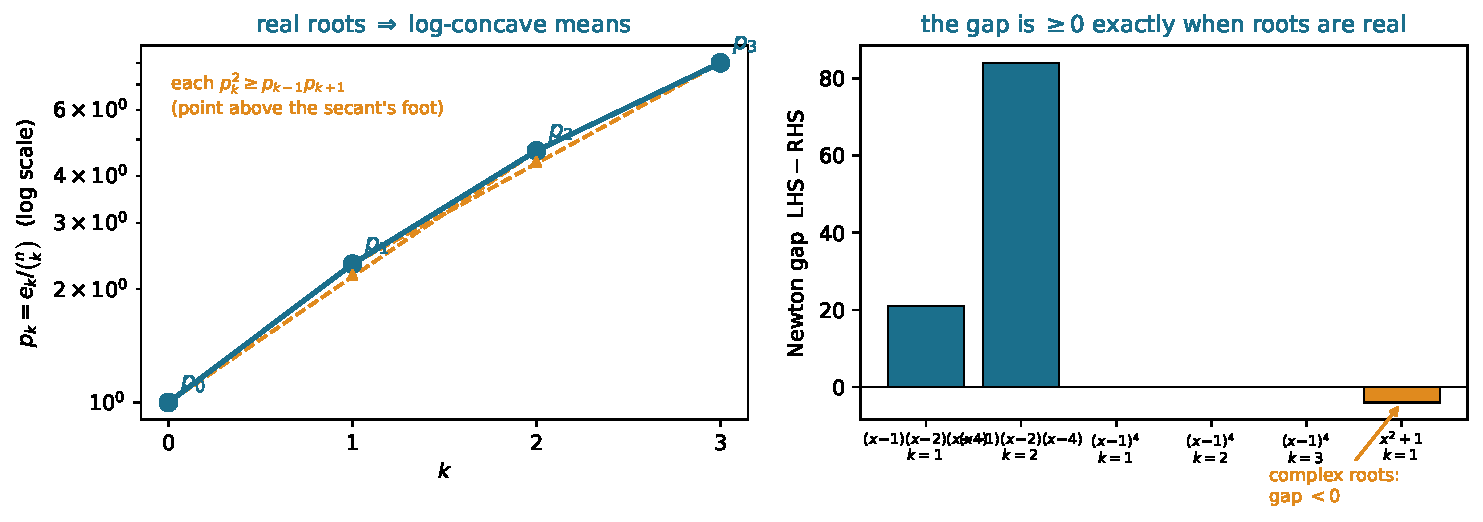
\includegraphics[width=0.92\textwidth]{newton_fig1_bow}
\caption{\emph{Izquierda:} las medias normalizadas de $(x-1)(x-2)(x-4)$, en eje logar\'itmico; cada
media interior queda por encima de la media geom\'etrica de sus vecinas (flechas \'ambar), as\'i que
la sucesi\'on es c\'oncava---``se arquea hacia dentro.'' \emph{Derecha:} la brecha de Newton
$e_k^2\binom{n}{k-1}\binom{n}{k+1}-e_{k-1}e_{k+1}\binom{n}{k}^2$ en cada $k$ interior: positiva para
la c\'ubica con ra\'ices reales, exactamente cero para $(x-1)^4$ (el caso afilado) y \emph{negativa}
para $x^2+1$. El script que la genera comprueba cada valor contra aritm\'etica entera exacta.}
\label{fig:bow}
\end{figure}

Un rasgo del enunciado merece una segunda mirada:
\begin{quote}\itshape
  ¿por qu\'e la diferencia entre ra\'ices reales y complejas aflora precisamente en las funciones
  sim\'etricas elementales, y precisamente como log-concavidad?
\end{quote}
Porque las $e_k$ \emph{son} los coeficientes del polinomio, le\'idos a trav\'es de Vieta, y la
real-radicalidad es una propiedad que se propaga hacia abajo por toda la torre de derivadas (Rolle)
y sobrevive a revertir el polinomio. Esos dos movimientos permiten aislar cualesquiera tres
coeficientes consecutivos como los coeficientes de una cu\'adratica con ra\'ices reales---y para una
cu\'adratica, ``con ra\'ices reales'' es literalmente ``discriminante $\ge0$.'' Esa es la
desigualdad de Newton, y la secci\'on siguiente es c\'omo una m\'aquina recorre el mismo camino.
\emph{¿Puede el gesto de libro de texto volverse una verificaci\'on de una l\'inea?}

\section{P2: ¿c\'omo se vuelve una verificaci\'on de una l\'inea para una m\'aquina?}\label{sec:proof}

\emph{Apunte hist\'orico.} La prueba por derivaci\'on--reversi\'on es la cl\'asica (Sylvester; el
relato en \cite{HLP}): muele el \'indice hasta una cu\'adratica usando operaciones que preservan la
realidad de las ra\'ices, e invoca el caso trivial $n=2$. Toda la cuesti\'on es si ``preserva
ra\'ices reales'' y ``reducir a una cu\'adratica'' sobreviven a hacerse plenamente formales.

\paragraph{Los objetos.} Trabajo sobre $\R$. Un polinomio tiene \emph{ra\'ices reales}
(\lean{RealRooted}) cuando se factoriza en factores lineales sobre $\R$---el \lean{Polynomial.Splits}
intr\'inseco de Mathlib; equivalentemente tiene $\deg p$ ra\'ices reales contadas con
multiplicidad. Para el multiconjunto de ra\'ices $s=p.\mathtt{roots}$, la funci\'on sim\'etrica
elemental es $e_k=\lean{Multiset.esymm}\,s\,k$, y $\binom{n}{k}=\lean{Nat.choose}$. Dos piezas de
Mathlib hacen de puente: \lean{coeff\_eq\_esymm\_roots\_of\_card} es Vieta,
$p.\mathtt{coeff}\,j=p.\mathtt{leadingCoeff}\cdot(-1)^{n-j}\,e_{n-j}$ (lo que me deja pasar entre el
enunciado en funciones sim\'etricas y uno en coeficientes), y \lean{card\_roots\_le\_derivative} es
Rolle para polinomios. Mathlib ten\'ia ambas mitades; no ten\'ia la desigualdad sobre ellas.

\paragraph{Las dos piedras.} Exactamente dos operaciones preservan la real-radicalidad y eso es todo
lo que la prueba necesita. \emph{Derivaci\'on:} entre ra\'ices reales consecutivas de $p$ hay una
ra\'iz real de $p'$ (Rolle), as\'i que $p'$ tiene $\ge\deg p-1$ ra\'ices reales, que es todas las
que puede tener (\lean{RealRooted.derivative}, iterada en \lean{RealRooted.iterate\_derivative}).
\emph{Reversi\'on:} $p^{\mathrm{rev}}$ es, salvo un factor no nulo, $p$ evaluado en $1/x$, as\'i que
sus ra\'ices son los rec\'iprocos de las ra\'ices no nulas de $p$, a\'un reales
(\lean{RealRooted.reverse}). Con ellas, la reducci\'on es corta.

\begin{recipebox}{La reducci\'on (receta)}
Para probar la desigualdad en el \'indice $i$ para un $p$ con ra\'ices reales de grado $n$ (sea
$N=n-i+1$): (1)~derivar $i-1$ veces: $q=p^{(i-1)}$, con ra\'ices reales y grado $N$;
(2)~revertir: $r=q^{\mathrm{rev}}$, con ra\'ices reales;
(3)~derivar $N-2$ veces: $g=r^{(N-2)}$, con ra\'ices reales y grado $\le2$.
Los tres coeficientes bajos de $g$ son \emph{m\'ultiplos factoriales} de $a_{i-1},a_i,a_{i+1}$
(escribiendo $a_j=p.\mathtt{coeff}\,j$), y el caso base
$g.\mathtt{coeff}\,1^2\ge4\,g.\mathtt{coeff}\,2\cdot g.\mathtt{coeff}\,0$ es, tras eliminar esos
factoriales positivos, la desigualdad de Newton en $i$.
\end{recipebox}

\begin{figure}[t]
  \centering
  \begin{tikzpicture}[node distance=4pt,
    box/.style={draw=ggteal,fill=ggband!40,rounded corners=2pt,inner sep=5pt,align=center,font=\small},
    arr/.style={-{Stealth[length=2.2mm]},ggteal,thick}]
    \node[box] (p) {$p=x^3-7x^2$\\$+14x-8$};
    \node[box,right=20pt of p] (q) {$q=p^{(0)}=p$\\\scriptsize($i{-}1{=}0$)};
    \node[box,right=20pt of q] (r) {$r=q^{\mathrm{rev}}$\\$=-8x^3{+}14x^2$\\$-7x{+}1$};
    \node[box,right=20pt of r] (g) {$g=r^{(1)}$\\$=-24x^2{+}28x{-}7$\\\scriptsize($N{-}2{=}1$)};
    \draw[arr] (p) -- (q);
    \draw[arr] (q) -- (r) node[midway,above,font=\scriptsize,ggteal]{revertir};
    \draw[arr] (r) -- (g) node[midway,above,font=\scriptsize,ggteal]{$d/dx$};
    \node[below=9pt of g,align=center,font=\small,text=ggamber] (disc)
      {discriminante $28^2-4(-24)(-7)$\\$=784-672=112\ge0$};
    \draw[arr,ggamber] (g) -- (disc);
    \node[below=8pt of q,align=center,font=\scriptsize,text width=8.7cm] {%
      cada flecha preserva la real-radicalidad, as\'i que $g$ es una cu\'adratica con ra\'ices
      reales y tiene discriminante no negativo. Eliminar factoriales positivos convierte
      $784\ge672$ en Newton en $i=1$: $a_1^2\binom{3}{0}\binom{3}{2}=588\ge
      a_0a_2\binom{3}{1}^2=504$ (proporcional, $\times\tfrac34$).};
  \end{tikzpicture}
  \caption{La reducci\'on derivar--revertir, trabajada en la c\'ubica de ejemplo en $i=1$
  (relacionando $a_0,a_1,a_2=-8,14,-7$). El objeto final es una cu\'adratica; una cu\'adratica con
  ra\'ices reales tiene discriminante no negativo; los factoriales que la prueba cancela son la
  constante de proporcionalidad.}
  \label{fig:reduction}
\end{figure}

\paragraph{El caso base, en coeficientes.} El coraz\'on $n=2$ es \lean{realRooted\_discrim\_coeff}:
un $q$ con ra\'ices reales y $\deg q\le2$ cumple $q.\mathtt{coeff}\,1^2\ge4\,q.\mathtt{coeff}\,2\cdot
q.\mathtt{coeff}\,0$. Se eval\'ua $q$ en una de sus ra\'ices $x$ y se lee
$b^2-4ac=(2ax+b)^2-4a(ax^2+bx+c)=(2ax+b)^2\ge0$. Enunciarlo sobre \emph{coeficientes}, con la
hip\'otesis d\'ebil $\deg\le2$, es la elecci\'on que mantiene limpia toda la prueba
(Secci\'on~\ref{sec:caught}).

\paragraph{La contabilidad.} La \'unica parte t\'ecnica es calcular los tres coeficientes bajos de
$g$. El \lean{coeff\_iterate\_derivative} de Mathlib da $(p^{(k)}).\mathtt{coeff}\,m=
(m{+}k)^{\underline{k}}\,p.\mathtt{coeff}(m{+}k)$ (un factorial descendente), y \lean{coeff\_reverse}
da $q^{\mathrm{rev}}.\mathtt{coeff}\,m=q.\mathtt{coeff}(\mathrm{revAt}\,(\deg q)\,m)$. Componer
derivar--revertir--derivar necesita el grado \emph{exacto} de cada intermedio, que sobre $\R$
(caracter\'istica cero, un anillo \lean{IsAddTorsionFree}) lo da \lean{degree\_derivative\_eq}:
derivar un polinomio de grado $d{>}0$ baja el grado en exactamente uno. Con los grados fijados, la
desigualdad del discriminante, tras reescribir cada factorial descendente v\'ia
$\lean{Nat.factorial\_mul\_descFactorial}$, queda
\keyeq{\bigl((N-1)!\,i!\bigr)^2\,a_i^2\;\ge\;N!\,(N-2)!\,(i-1)!\,(i+1)!\;a_{i-1}a_{i+1},}
y la identidad binomial $\binom{n}{k}\,k!\,(n-k)!=n!$
(\lean{Nat.choose\_mul\_factorial\_mul\_factorial}) elimina esos factores positivos para casar con
el Teorema~\ref{thm:newton}---sin razonamiento de desigualdades, solo positividad. La forma en
funciones sim\'etricas se sigue de la forma en coeficientes (\lean{newton\_inequality\_coeff}) por
Vieta, cancelando los signos $(-1)^{k-1}(-1)^{k+1}=1$ y reindexando los binomios por
$\binom{n}{k}=\binom{n}{n-k}$ al \'indice $i=n-k$.

As\'i que la respuesta a P2 es s\'i: la desigualdad se reduce, en tres movimientos que preservan la
realidad, a un \'unico discriminante que la m\'aquina cierra por \lean{sq\_nonneg}. \emph{Y en el
\'unico punto donde el libro de texto agita la mano, la m\'aquina me lo hizo ganar.}

\section{P3: ¿qu\'e caz\'o la m\'aquina que el libro de texto pasa por alto?}\label{sec:caught}

\emph{Apunte hist\'orico.} ``Derivar, revertir, reducir a una cu\'adratica'' es como corre la prueba
cl\'asica, y la prueba cl\'asica supone calladamente que el polinomio revertido conserva su grado.
Un asistente de pruebas no deja pasar la suposici\'on sin examinarla---y examinarla \emph{quit\'o} un
caso aparte, no lo a\~nadi\'o.

El paso de reversi\'on preserva el \emph{grado} solo cuando el coeficiente l\'ider del polinomio
revertido es no nulo, lo que falla exactamente cuando $a_{i-1}=0$. El reflejo de libro de texto es un
caso aparte: tratar $a_{i-1}=0$ por separado. Lo evito por completo, y la raz\'on es la forma del
caso base.

\begin{recipebox}{Para qu\'e sirve de verdad un asistente de pruebas}
Enunciar el caso base sobre \emph{coeficientes} con la hip\'otesis d\'ebil $\deg\le2$ (no $=2$) hace
que devuelva un enunciado verdadero incluso cuando la cu\'adratica degenera: si
$g.\mathtt{coeff}\,2=0$ la desigualdad dice $g.\mathtt{coeff}\,1^2\ge0$, que es \lean{sq\_nonneg}.
Rastre\'andolo, cuando $a_{i-1}=0$ el lado derecho de Newton es $a_{i-1}a_{i+1}\binom{n}{i}^2=0$ y el
izquierdo es un cuadrado por binomios no negativos---as\'i que la desigualdad se cumple por una
raz\'on ajena a la cu\'adratica. \emph{La maquinaria general y el caso degenerado se cierran con la
misma l\'inea.} La lecci\'on transferible: elegir la hip\'otesis honesta m\'as d\'ebil para un caso
base a menudo disuelve los casos l\'imite que un enunciado m\'as afilado te obligar\'ia a perseguir.
\end{recipebox}

Esto es todo lo que la formalizaci\'on a\~nadi\'o m\'as all\'a de la transcripci\'on, y es
honestamente peque\~no---no un teorema sino una disciplina. Es tambi\'en exactamente el tipo de paso
que justifica verificar por m\'aquina un resultado que todos ya creen: el lugar donde ``sin p\'erdida
de generalidad'' resulta no costar nada, pero solo una vez que se ha mirado. \emph{Con Newton
certificado, ¿qu\'e obtiene gratis el resto de esta l\'inea de trabajo?}

\section{P4: con Newton certificado, ¿qu\'e sale gratis?}\label{sec:corollaries}

\emph{Apunte hist\'orico.} La implicaci\'on ``ra\'ices reales $\Rightarrow$ coeficientes
log-c\'oncavos'' es el caballo de batalla del \'area: es por lo que los n\'umeros de emparejamientos
de un grafo son log-c\'oncavos (v\'ia Heilmann--Lieb~\cite{PartII}), por lo que lo son los
coeficientes del polinomio de independencia de un grafo sin garras, y la mitad f\'acil de los
resultados que, para matroides, necesitaron teor\'ia de Hodge porque no hab\'ia polinomio con
ra\'ices reales~\cite{AHK2018}.

El lema en forma de coeficientes \lean{newton\_inequality\_coeff} est\'a enunciado precisamente para
que aliment\'andolo con cualquier polinomio con ra\'ices reales rinda la log-concavidad de los
coeficientes de ese polinomio, sin m\'as trabajo:
\keyeq{\text{ra\'ices reales}\;\Longrightarrow\;\text{coeficientes log-c\'oncavos}.}
El polinomio de emparejamientos de un grafo tiene ra\'ices reales (Heilmann--Lieb, el art\'iculo
anterior de esta l\'inea~\cite{PartII}); componerlo con el lema probado aqu\'i da la log-concavidad
de los n\'umeros de emparejamientos como corolario inmediato, en vez del gesto de libro de texto que
ha sido a lo largo de esta serie. La misma l\'inea sirve para cualquier polinomio con ra\'ices
reales que un desarrollo en Lean produzca en el futuro.

Dos caminos se abren directamente hacia arriba (la Tabla~\ref{tab:inventory} lista lo construido;
estos son lo que a\'un no):
\begin{itemize}\itemsep1pt
\item \textbf{Las desigualdades de medias de Maclaurin} $p_1\ge p_2^{1/2}\ge\cdots\ge p_n^{1/n}$,
  consecuencia hist\'orica inmediata de Newton---ahora un objetivo concreto y no una cita.
\item \textbf{Los casos de igualdad}: que la igualdad en un $k$ interior fuerza que todas las
  ra\'ices sean iguales, el compa\~nero afilado cl\'asico, visible en la fila $(x-1)^4$ de la
  Figura~\ref{fig:bow} pero a\'un no probado.
\end{itemize}

Una pregunta que vale la pena llevarse:
\begin{quote}\itshape
  ¿por qu\'e dos operaciones tan distintas como \emph{derivar} y \emph{tomar rec\'iprocos de las
  ra\'ices} preservan ambas la realidad de las ra\'ices---y por qu\'e ese par basta exactamente para
  exponer cada ventana de coeficientes?
\end{quote}
Porque ambas son sombras de un mismo hecho: los polinomios con ra\'ices reales forman un mundo
cerrado (su casa en varias variables son los polinomios estables de Br\"and\'en~\cite{Branden2015}).
La derivaci\'on es el operador lineal m\'as simple que lo preserva, la reversi\'on la involuci\'on
m\'as simple; entre ambas act\'uan sobre las ventanas de coeficientes con transitividad suficiente
para hacer aflorar cualesquiera tres coeficientes consecutivos como una cu\'adratica. Las
desigualdades de Newton son la primera consecuencia visible de esa clausura---y la reducci\'on de
este art\'iculo es, en miniatura, c\'omo todo argumento posterior de real-radicalidad toma prestada
su fuerza.

\section{Los bloques de construcci\'on}\label{sec:blocks}

El resultado principal descansa en cuatro piezas reutilizables---la salida genuinamente
portable---cada una libre de \lean{sorry} con los tres axiomas est\'andar
(Tabla~\ref{tab:inventory}).

\begin{lemma}[\lean{RealRooted.derivative}, \lean{RealRooted.iterate\_derivative}]
Si $p$ tiene ra\'ices reales entonces $p'$ tambi\'en, y por tanto toda derivada iterada $p^{(k)}$.
\end{lemma}
El teorema de Rolle para polinomios (\lean{card\_roots\_le\_derivative}) apretado contra la ca\'ida
de grado: $p'$ ya tiene $\deg p-1$ ra\'ices reales, que es lo m\'as que puede tener.

\begin{lemma}[\lean{RealRooted.reverse}]
Si $p$ tiene ra\'ices reales entonces su reversi\'on $p^{\mathrm{rev}}$ tambi\'en.
\end{lemma}
Factorizando $p$ en lineales m\'onicos y revirtiendo cada uno; la hip\'otesis sobre el t\'ermino
constante que el libro de texto le adosa es \emph{innecesaria} y se elimina---la reversi\'on solo
descarta ceros de cola, y el producto restante de factores de grado $\le1$ a\'un se factoriza.

\begin{lemma}[\lean{realRooted\_discrim\_coeff}]
Un $q$ con ra\'ices reales y $\deg q\le2$ cumple $q.\mathtt{coeff}\,1^2\ge4\,q.\mathtt{coeff}\,2\cdot
q.\mathtt{coeff}\,0$.
\end{lemma}
El caso base de la reducci\'on, en forma de coeficientes; la fuente del caso aparte disuelto
(Secci\'on~\ref{sec:caught}).

\begin{table}[h]
\centering\small
\rowcolors{2}{ggband!35}{white}
\begin{tabular}{@{}lll@{}}
\toprule
\rowcolor{ggteal!18} Nombre Lean & enunciado & papel \\
\midrule
\lean{newton\_inequality} & $e_k^2\binom{n}{k-1}\binom{n}{k+1}\ge e_{k-1}e_{k+1}\binom{n}{k}^2$ & Teorema~\ref{thm:newton} \\
\lean{newton\_logConcave} & $p_{k-1}p_{k+1}\le p_k^2$ (medias normalizadas) & corolario \\
\lean{newton\_inequality\_coeff} & $a_i^2\binom{n}{i-1}\binom{n}{i+1}\ge a_{i-1}a_{i+1}\binom{n}{i}^2$ & forma en coef. \\
\lean{realRooted\_discrim\_coeff} & ra\'ices reales, $\deg\le2\Rightarrow a_1^2\ge4a_2a_0$ & caso base \\
\lean{RealRooted.derivative} & $p$ con ra\'ices reales $\Rightarrow p'$ id. & bloque (Rolle) \\
\lean{RealRooted.iterate\_derivative} & $p$ con ra\'ices reales $\Rightarrow p^{(k)}$ id. & bloque \\
\lean{RealRooted.reverse} & $p$ con ra\'ices reales $\Rightarrow p^{\mathrm{rev}}$ id. & bloque \\
\bottomrule
\end{tabular}
\caption{Los resultados que cargan peso, todos libres de \lean{sorry} en \lean{Newton.lean} del
repositorio (346 l\'ineas, sobre \lean{RealStable.lean} y Mathlib). Axiomas de cada entrada:
\lean{propext}, \lean{Classical.choice}, \lean{Quot.sound} solamente; sin \lean{native\_decide}, sin
axioma propio.}
\label{tab:inventory}
\end{table}

\section{El l\'imite de la contribuci\'on}\label{sec:boundary}

Todo lo que aqu\'i son matem\'aticas es cl\'asico: Newton (1707), Maclaurin (1729), la prueba de
Sylvester, el tratamiento de libro de texto en Hardy--Littlewood--P\'olya~\cite{HLP}. No reclamo
identidad ni desigualdad nuevas. Las contribuciones son tres: la \emph{formalizaci\'on} (hasta donde
s\'e, la primera prueba verificada por m\'aquina de las desigualdades de Newton en cualquier
asistente de pruebas); la \emph{infraestructura reutilizable}---real-radicalidad bajo derivaci\'on,
derivaci\'on iterada y reversi\'on, y el discriminante en forma de coeficientes---que es justo lo que
cualquier desarrollo posterior de real-radicalidad o estabilidad en Mathlib querr\'a; y el
\emph{registro de ingenier\'ia de pruebas} de la Secci\'on~\ref{sec:caught}, el caso base de
hip\'otesis d\'ebil que disuelve un caso aparte.

\emph{Alcance, dicho con claridad.} Pruebo las desigualdades \emph{sobre $\R$}---la casa natural de
la real-radicalidad, y lo que usa la reducci\'on---no sobre un cuerpo real-cerrado u ordenado
abstracto, aunque nada en el argumento se resiste a ello. Pruebo la desigualdad y su corolario de
log-concavidad, \emph{no} el an\'alisis de igualdad/estrictez (la igualdad fuerza que todas las
ra\'ices sean iguales), ni la cadena de medias de Maclaurin: esos est\'an mapeados
(Secci\'on~\ref{sec:corollaries}), no construidos.

\emph{Formalizaciones previas.} La reclamaci\'on de prioridad descansa en una b\'usqueda
documentada, no en una corazonada. Para las desigualdades de Newton y las funciones sim\'etricas
elementales busqu\'e (junio de 2026): Mathlib (Loogle y \lean{grep}---\lean{Multiset.esymm} y las
relaciones de Vieta existen; \emph{Maclaurin} y las desigualdades de \lean{esymm} al cuadrado no),
los repositorios m\'as amplios de la comunidad Lean, el Archive of Formal Proofs de Isabelle y el
ecosistema Coq/Rocq. Ninguno contiene las desigualdades de Newton. Como siempre, tal reclamaci\'on
se hace hasta donde alcanza mi conocimiento.

\emph{Sobre la metodolog\'ia.} La formalizaci\'on se hizo con un asistente de IA (Claude, Anthropic),
bajo la disciplina de los art\'iculos compa\~neros: la aritm\'etica de la reducci\'on verificada
num\'ericamente antes de formalizar (\lean{figures/newton\_fig1\_bow.py} recomprueba cada instancia),
y cada teorema con nombre verificado por \lean{\#print axioms} para depender solo de \lean{propext},
\lean{Classical.choice}, \lean{Quot.sound}. La correcci\'on no descansa en el asistente: el n\'ucleo
de Lean comprueba toda prueba. La contabilidad cuidadosa---el alcance sobre $\R$ dicho tan
claramente como el resultado, los casos de igualdad dejados expl\'icitamente abiertos---es parte de
lo que el m\'etodo, en su mejor versi\'on, deber\'ia producir. Las matem\'aticas y las afirmaciones
son responsabilidad del autor.

\section{Preguntas abiertas}\label{sec:questions}

Las desigualdades de Newton son ya un teorema en la biblioteca. Los objetivos concretos
siguientes---la cadena de medias de Maclaurin, los casos de igualdad, la log-concavidad de los
n\'umeros de emparejamientos---est\'an nombrados en la Secci\'on~\ref{sec:corollaries}; lo que sigue
son las preguntas que prefiero llevarme a marcar como tareas, una por giro del argumento, la \'ultima
la que me quedar\'ia.

\begin{enumerate}
\item \emph{Por qu\'e los ceros se vuelven magnitudes.} La realidad de las ra\'ices es un enunciado
sobre \emph{d\'onde} se anula un polinomio; la log-concavidad, sobre el \emph{tama\~no} de sus
coeficientes. Newton es el primer puente, y el m\'as barato, entre ambos. ¿Cu\'al es la raz\'on m\'as
profunda de que una restricci\'on sobre los ceros de un polinomio se convierta, ventana a ventana, en
una restricci\'on sobre la magnitud de sus coeficientes?
\item \emph{La jerarqu\'ia de certificados.} Para una sucesi\'on de reales no negativos, la
real-radicalidad del polinomio generador equivale a ser una sucesi\'on de frecuencia de P\'olya
(Aissen--Schoenberg--Whitney), estrictamente m\'as fuerte que la log-concavidad (que es
$\mathrm{PF}_2$). Newton deduce el extremo d\'ebil del fuerte. ¿Qu\'e vive exactamente en la brecha
entre los pelda\~nos, y hay un certificado \emph{m\'as barato} para cada uno que un asistente de
pruebas pudiera aprender a elegir?
\item \emph{La clausura, explicitada.} La derivaci\'on y la reversi\'on preservan cada una la
real-radicalidad, y ese par ya basta para exponer cualesquiera tres coeficientes consecutivos como
una cu\'adratica. ¿Cu\'al es el monoide completo de operaciones sobre ventanas de coeficientes que
preservan la real-radicalidad, y es ``alcanza toda ventana cu\'adratica'' un teorema que se pueda
enunciar y verificar---esto es, es la suficiencia de \emph{estas dos} piedras un teorema en s\'i?
\item \emph{Por encima del suelo con ra\'ices reales.} Donde no existe polinomio con ra\'ices
reales---matroides---la log-concavidad necesita teor\'ia de Hodge~\cite{AHK2018}, con los polinomios
lorentzianos de Br\"and\'en interpolando entre ambos mundos. ¿Es Newton la sombra en una variable de
la lorentzianidad, y cu\'al es el fragmento formalizado m\'as peque\~no que lo har\'ia un piso de un
mismo edificio en vez de un hecho cl\'asico aislado?
\item \emph{Una para quedarse.} Lo \'unico que la formalizaci\'on a\~nadi\'o m\'as all\'a de la
transcripci\'on fue que la hip\'otesis de caso base \emph{m\'as d\'ebil y honesta} disolvi\'o un caso
aparte (Secci\'on~\ref{sec:caught})---el ``sin p\'erdida de generalidad'' no cost\'o nada, pero solo
una vez que una m\'aquina me hizo mirar. En una teor\'ia de tres siglos y reprobada muchas veces,
¿con qu\'e frecuencia es gratis ese ``sin p\'erdida'', y es ``busca siempre la hip\'otesis base m\'as
d\'ebil'' un principio transferible de la prueba mec\'anica o un accidente feliz de esta?
\end{enumerate}

\section*{Reproducir}
\begin{verbatim}
git clone https://github.com/karlesmarin/godsil-gutman-lean
cd godsil-gutman-lean && lake exe cache get
lake env lean Newton.lean
\end{verbatim}
Lean \lean{v4.30.0-rc2}, pin de Mathlib \lean{701fb6e9}. Los teoremas son
\lean{Newton.newton\_inequality}, \lean{newton\_logConcave} y \lean{newton\_inequality\_coeff} en
\lean{Newton.lean}; sus soportes est\'an en la Tabla~\ref{tab:inventory}. Cada uno se comprueba por
\lean{\#print axioms} y depende solo de \lean{propext}, \lean{Classical.choice}, \lean{Quot.sound}.
La figura se regenera con \lean{python figures/newton\_fig1\_bow.py}, que comprueba su contenido
contra aritm\'etica exacta antes de dibujar.

\begin{thebibliography}{99}\small
\bibitem{Newton1707} I.~Newton, \emph{Arithmetica Universalis} (1707); las desigualdades entre los
coeficientes de un polinomio con ra\'ices reales se enuncian all\'i sin prueba.
\bibitem{Maclaurin1729} C.~Maclaurin, A second letter \dots\ concerning the roots of equations,
with the demonstration of other rules in algebra, \emph{Phil.\ Trans.\ Roy.\ Soc.\ London}
\textbf{36} (1729) 59--96.
\bibitem{HLP} G.~H.~Hardy, J.~E.~Littlewood, G.~P\'olya, \emph{Inequalities}, 2.\textsuperscript{a}
ed., Cambridge Univ.\ Press, 1952 (desigualdades de Newton y Maclaurin, \S2.22).
\bibitem{Stanley1989} R.~P.~Stanley, Log-concave and unimodal sequences in algebra,
combinatorics, and geometry, \emph{Ann.\ New York Acad.\ Sci.} \textbf{576} (1989) 500--535.
\bibitem{Branden2015} P.~Br\"and\'en, Unimodality, log-concavity, real-rootedness and beyond, en
\emph{Handbook of Enumerative Combinatorics}, CRC Press, 2015, 437--483.
\bibitem{AHK2018} K.~Adiprasito, J.~Huh, E.~Katz, Hodge theory for combinatorial geometries,
\emph{Ann.\ of Math.} \textbf{188} (2018) 381--452.
\bibitem{PartI} C.~Mar\'in, \emph{Random Signs into Matchings: A Godsil--Gutman Identity,
Formalized in Lean~4}, Zenodo, 2026. \texttt{doi:10.5281/zenodo.20517350}.
\bibitem{PartII} C.~Mar\'in, \emph{Unfolding a Graph into a Tree: A Machine-Checked Proof of the
Heilmann--Lieb Theorem in Lean~4}, Zenodo, 2026.
\texttt{https://github.com/karlesmarin/godsil-gutman-lean}.
\bibitem{Mathlib2020} The mathlib Community, The Lean mathematical library, en \emph{CPP 2020},
ACM, 2020, 367--381.
\end{thebibliography}

\end{document}
